\chapter{Implementation of the method for unidirectional waves}
The present section gives a short introduction to the analysis method by presenting the utilized JONSWAP spectrum parameters, the definition of the Fourier series and the model parameters used in the report. 
\section{Background}
The JONSWAP spectrum is defined as
\begin{subequations}
\begin{equation}
    S_{\eta \eta}(f) = \alpha H_s^2 f_p^4 f^{-5} \gamma^\beta \exp{\left[-\frac{5}{4}\left(\frac{f_p}{f}\right)^4\right]}
    \label{eq:JONSWAPSpec}
\end{equation} 
\begin{equation}
    \alpha =\frac{0.0624}{0.230+0.0336\gamma-\frac{0.185}{1.9+\gamma}} ,\quad \beta = \exp{\left[ -\frac{(f-f_p)^2}{2\sigma^2f_p^2} \right]}, \quad
    \sigma =
    \begin{cases}
    0.07, \quad \text{for }f\leq f_p \\
    0.09, \quad \text{for }f> f_p
    \end{cases},
    \label{eq:JONSWAPparam}
\end{equation}
\label{eq:JONSWAP}
\end{subequations}
where \cref{eq:JONSWAPSpec} defines the power spectrum and \cref{eq:JONSWAPparam} defines the suggested scalar parameters given in the slides. Here, $H_s$ is the significant wave height, $f_p$ is the frequency corresponding to the peak period (i.e. $f_p=1/T_p$), $f$ is the frequency of interest, $\gamma$ is the so-called peak enhancement factor and $\alpha$, $\beta$, $\sigma$ are scalar parameters describing the shape of the JONSWAP spectrum. 

The irregular wave series can be expressed using a Fourier series, where the standard Fourier representation can be written as
\begin{equation}
    \eta(t) = \sum_{n=1}^{n_{\text{max}}} a_n \cos{(\omega_n t)} +b_n \sin{(\omega_n t)}, \quad \text{where }\omega_n=\frac{2\pi}{T_n} \  \text{and} \ f_n=n\,df
\end{equation}
here $a_n$ and $b_n$ are the unknown Fourier coefficients, and $\omega_n$, $T_n$ and $f_n$ is the angular wave frequency, wave period, and wave frequency of each wave component, respectively. The equivalent complex representation can be formulated as
\begin{equation}
    \eta(t,x) = \sum_{n=1}^{n_{\text{max}}} c_n e^{-i(\omega_n t-k_n x)} + \Tilde{c}_n e^{i(\omega_n t - k_n x)}, \quad \text{where }c_n=\frac{1}{2}(a_n+i b_n) \ \text{and} \ \Tilde{c}_n=\frac{1}{2}(a_n-i b_n)
    \label{eq:ComplexFourier}
\end{equation}
which is valid as the function wave function, $\eta$, only has physical meaning for real values, i.e. $c_{-n}=\Tilde{c}_n$. \cref{eq:ComplexFourier} also shows the conversion between the real and complex Fourier coefficients. Note that the actual wave surface elevation is the real part of the above complex representation, and that the tilde $[\, \Tilde{\text{\scalebox{0.5}{\textbullet}}}\,]$ denotes the complex conjugate.

\begin{table}[h]
    \centering
    \caption{Model parameters (Group 10)}
    \begin{tabular}{@{}lllll@{}}
    \toprule
    Significance                            &   Symbol          & Unit       & Value \\ \hline
    Water depth                             &   $h$             & \si{m}     & 29   \\
    Significant wave height                 &   $H_{s}$         & \si{m}     & 6.75   \\
    Peak wave period                        &   $T_p$           & \si{s}     & 11.5  \\ \addlinespace[1mm]
    Peak enhancement factor                 &   $\gamma$        & \si{-}     & 3.0 \\ \addlinespace[1mm]
    Spreading factor                        &   $s$             & \si{-}     & 2.75   \\ \addlinespace[1mm]
    Duration of wave conditions             &   $t_{\text{dur}}$& \si{s}     & 3600   \\
    Time step size                          &   $dt$            & \si{s}     & 0.25   \\
    \bottomrule
    \end{tabular}
    \label{tab:Modelparameters}
\end{table}

\section{Implementation for unidirectional waves}

The first step in generating the wave time series is to compute the power spectrum, $S_{\eta \eta}(f)$, using the previously defined JONSWAP spectrum (\cref{eq:JONSWAP}). The JONSWAP spectrum is implemented into a MATLAB function denoted \verb+JONSWAP(Hs,fp,gam,fvec)+, which outputs the JONSWAP spectrum. The inputs are given (in order) as the significant wave height, the peak frequency, the peak enhancement factor and a vector containing the frequency discretization. The frequency discretization vector contains frequencies up to the Nyquist frequency, $f_{\text{Nyq}}(=\frac{1}{2dt})$, with the step size determined by the bandwidth of the frequency resolution, $df(=\frac{1}{t_{\text{dur}}})$, i.e. \verb+fvec+$=\{df\ 2df \ \dots \ f_{\text{Nyq}}\}^T$.

Having obtained the power spectrum up until the Nyquist frequency, the second step is to provide an estimate for the phase shift of each component, $\delta_n$. As this is phase angle cannot be determined from the spectrum, $S_{\eta \eta}(f)$, the usual procedure is to assume that $\delta_n$ is a uniformly distributed stochastic variable over the interval $0<\delta_n\leq 2\pi$. The uniform distribution is achieved using the MATLAB intrinsic (pseudo) random number generator \verb+rand()+, with a fixed seed for reproducibility (seed=100).

The third step is to determine the complex conjugate pair of Fourier coefficients $\{c_n,\ \Tilde{c_n}\}$. This is achieved by first determining the real Fourier coefficients using the relations
\begin{equation}
    A_n = \sqrt{2 S_{\eta \eta}(f_n)\,df}, \quad a_n=A_n\cos{(\delta_n)}, \quad b_n=A_n\sin{(\delta_n)}
\end{equation}
and then converting $\{a_n,\ b_n \}$ (using \cref{eq:ComplexFourier}) to the paired complex coefficients, $\{c_n,\ \Tilde{c}_n\}$.

The fourth step is more easily understood when first introducing a new coefficient, $d_n$, such that \cref{eq:ComplexFourier} can be written as
\begin{equation}
        \eta(t,x) = \sum_{n=1}^{n_{\text{max}}} d_n e^{-i\omega_n t} + \Tilde{d}_n e^{i\omega_n t}
    \label{eq:ComplexFourier2}, \quad d_n = c_n e^{ik_n x}, \qquad \Tilde{d}_n = \Tilde{c}_n e^{-ik_n x}.
\end{equation}
which is exactly what the Inverse Discrete Fourier Transform (IDFT) computes for a set of data points in a large matrix multiplication, requiring $O(n^2)$ multiplication operations. However, the computational efficiency can be greatly improved by using the Inverse Fast Fourier Transform (IFFT) that only requires $O(n\log{(n)})$ multiplication operations.
\begin{figure}[htbp]
    \centering
    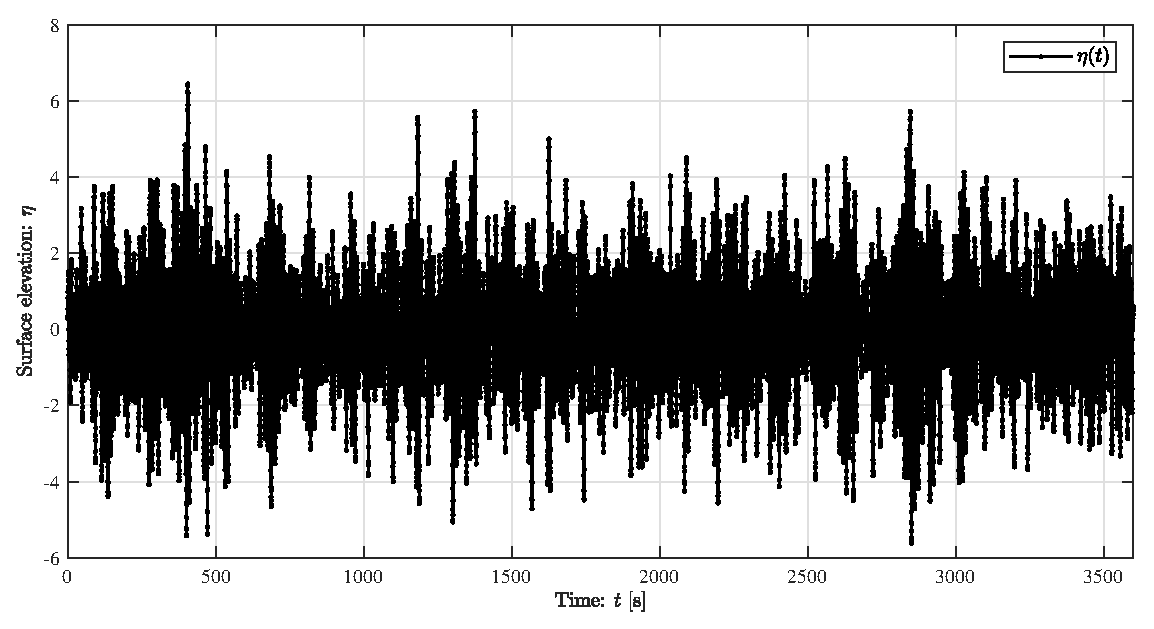
\includegraphics[width=0.9\textwidth]{Figures/Plots/SurfaceElevation.eps}
    \caption{Free surface elevation as a function of time, $\eta(t)$, generated from the JONSWAP spectrum using the Fast Fourier Transform (FFT) method.}
    \label{fig:SurfaceElevation}
\end{figure}

Thus, the fourth step revolves around arranging the Fourier coefficients in the correct order for the MATLAB IFFT algorithm, \verb+ifft()+. As previously mentioned, the desired discrete surface elevation function must only contain real values, making the coefficients conjugate symmetric ($c_{-n}=\Tilde{c}_n$). Thus, the coefficients, $d_n$, are also conjugate symmetric, and MATLAB requires the input vector to the \verb+ifft()+ function (here denoted $d_{FFT}^\eta$) to be stored in a \textit{wrap-around} order in the vector, such as
\begin{equation}
    d_{FFT}^\eta = [\, \Bar{\eta}\ d_1\ d_2\ \dots \ d_{(N_{Nyq}-1)} \ d_{N_{Nyq}} \ \Tilde{d}_{N_{Nyq}} \ \Tilde{d}_{(N_{Nyq}-1)} \ \dots \  \Tilde{d}_2 \ \Tilde{d}_1 \ \Bar{\eta} \, ], 
    \label{eq:dfftvector}
\end{equation} 
here $\Bar{\eta}$ is the mean wave height (set to zero) and $N_{Nyq}$ is the index of the Nyquist frequiency, $f_{Nyq}$. Finally, inserting the vector, $d_{FFT}^\eta$, into the \verb+ifft()+ function with the \verb+symmetric+ option enabled results in the surface elevation time series illustrated in \cref{fig:SurfaceElevation}. 

\vspace{15mm}
{\let\clearpage\relax \chapter{Analyzing the implementation}}

The purpose of the present section is to analyze the wave series generated from the wave characteristics and the JONSWAP spectrum (\cref{fig:SurfaceElevation}), with the goal of validating the implementation. The analysis is split into small steps following the order given in the problem description.

\paragraph{2.a)} The zero-moment of the spectral description is presented below in both a continuous and discrete from as
\begin{equation}
    m_0 = \int_0^\infty S_{\eta \eta}(f) \dif f, \qquad m_0 = \sum_{n=1}^{n_{max}} S_{\eta\eta}(f)\,df,
\end{equation}
which evaluates to $m_0=\SI{2.84}{m^2}$ when applying the discrete formulation to the output of the previously computed JONSWAP spectrum. This number, which represents the area under the JONSWAP spectrum curve, is difficult to asses from the plot but it is necessary to compute the significant wave height from the spectrum, $H_{m0}$.
\squeezeup
\paragraph{2.b)} The significant wave height from the spectrum, $H_{m0}$, is found using the expression $H_{m0} = 4\sqrt{m_0}$. This results in a significant wave height of $H_{m0}=\SI{6.74}{m}$, representing a relative deviation of $\SI{-0.16}{\percent}$ from the initial significant wave height, $H_s=\SI{6.75}{m}$ (\cref{tab:Modelparameters}). The difference is attributed to the (pseudo-random) introduction of the phase components, $\delta_n$, which causes random wave interference. Thus, the JONSWAP spectrum seems to be implemented correctly. 

\paragraph{2.c)} The specific implementation of the zero-down crossing analysis is summarised by the following three steps
\begin{enumerate}
    \item Identify zero-down crossings by checking: $\eta_{(i-1)}> 0$ and $\eta_{i} < 0$, for all $\eta_i$ and store indices
    \item Perform linear interpolation of the wave periods to zero wave height
    \item Find zero-down crossing wave heights: $H_k^{\text{zdc}}=\max(\eta_{j})-\min(\eta_{j})$, for $j$ going between all of the stored indices found in step 1.
\end{enumerate}
The significant wave height from the zero-down crossing analysis is then found by computing the mean of the 2/3 quantile, $q_{0.667}$, of the obtained zero down crossing wave heights. This results in a significant wave height of $H_s^{zdc}=\SI{6.56}{m}$, which gives a relative deviation of $\SI{-2.8}{\percent}$ from the input significant wave height (\cref{tab:Modelparameters}). \textcolor{red}{DISCUSS?}

\paragraph{2.d)} \Cref{fig:etaIFFTDistributions} illustrates the empirical distribution of the generated surface elevations (\cref{fig:SurfaceElevation}). \Cref{fig:etaIFFTHist} compares the empirical probalility density function with the equivalent normal distribution (based on the sample mean and sample variance), and \Cref{fig:etaIFFTqqplot} is a quantile-quantile plot (Q-Q plot) of the surface elevations versus the standard normal distribution. The figures generally illustrates good agreement with the expected normally distributed surface elevations. However, it is observed that there are some deviations from normality at the tails of the distribution (\cref{fig:etaIFFTqqplot}).\textcolor{red}{WHY does the surface elevation follow a normal distribution}. 

To evaluate the distribution quantitatively, the skewness, $s_k$, and kurtosis, $k_u$, are computed and compared to the expected values for a normal distribution, i.e. $s_k=0$, and $k_u=3$. The skewness and kurtosis for the continuous case can be defined as
\begin{equation}
    s_k = \frac{1}{\sigma^3}\frac{1}{T_0}\int_0^{T_0} (\eta(t)-\Bar{\eta})^3 \dif t, \quad k_u = \frac{1}{\sigma^4}\frac{1}{T_0}\int_0^{T_0} (\eta(t)-\Bar{\eta})^4 \dif t.
\end{equation}
where $\Bar{\eta}$ is the mean of the surface elevation, and $\sigma$ is the variance of the surface elevation. Computing the skewness and kurtosis yields $s_k=-0.02$ and $k_u=2.92$, respectively. Hence, the surface elevation again seems to approximately follow a normal distribution.

\begin{figure}[htb]
\begin{subfigure}[t]{.5\textwidth}
    \centering
    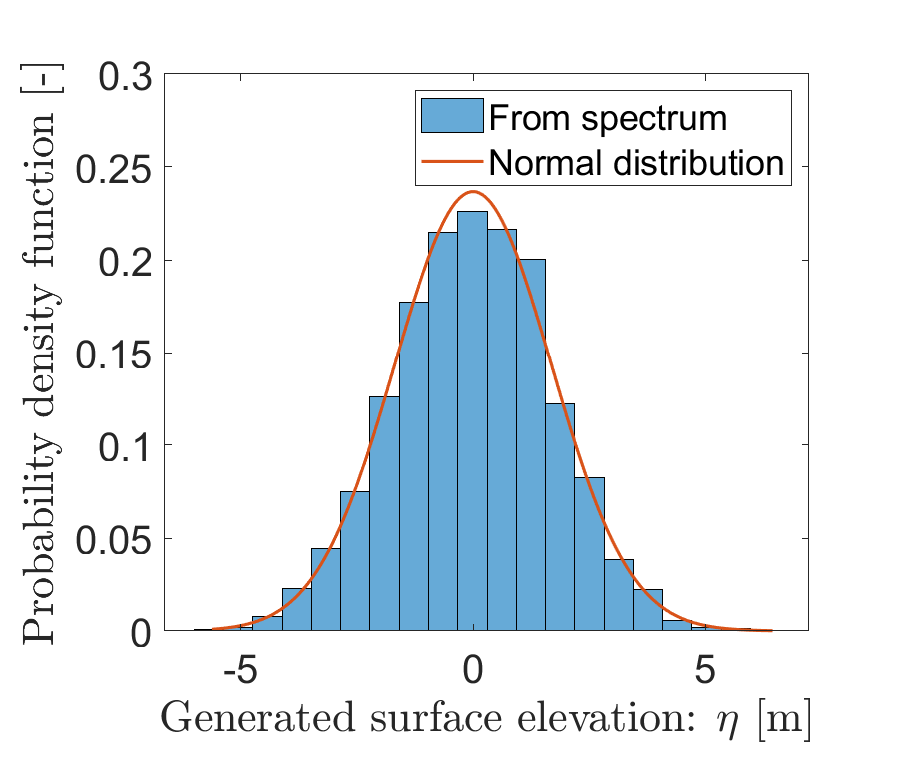
\includegraphics[width=.95\textwidth,trim=0cm 0cm 0.0cm 0cm, clip=true]{Figures/Plots/etaIFFTdist}
    \caption{Empirical probability density function}
    \label{fig:etaIFFTHist}
\end{subfigure}%
\begin{subfigure}[t]{.5\textwidth}
    \centering
    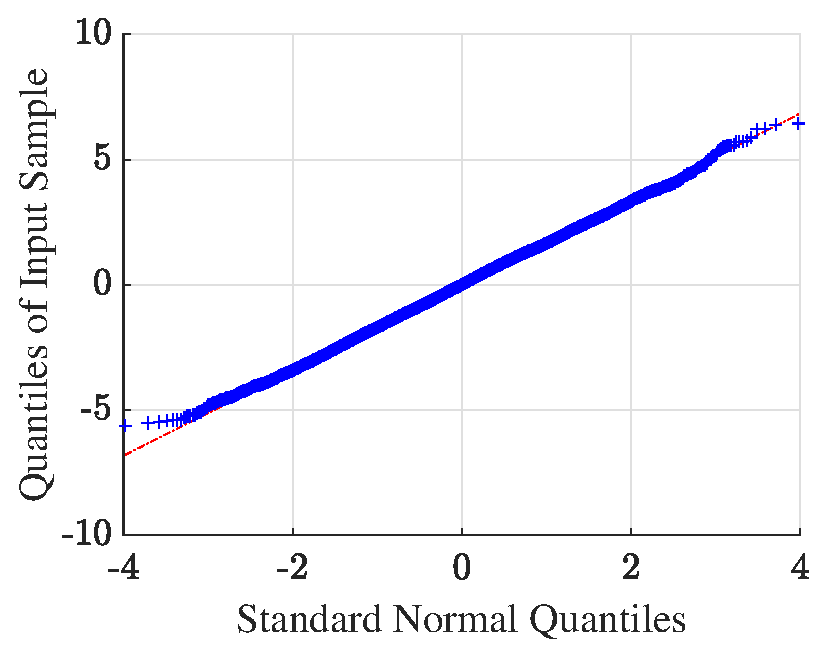
\includegraphics[width=0.95\textwidth,trim=0cm 0cm 0cm 0cm, clip=true]{Figures/Plots/etaIFFqqplot}
    \caption{Q-Q plot of surface elevations versus standard normal}
    \label{fig:etaIFFTqqplot}
\end{subfigure}
\caption{Empirical distribution of the generated surface elevations, $\eta$, shown in \cref{fig:SurfaceElevation}.}
\label{fig:etaIFFTDistributions}
\end{figure}

\begin{figure}[htbp]
    \centering
    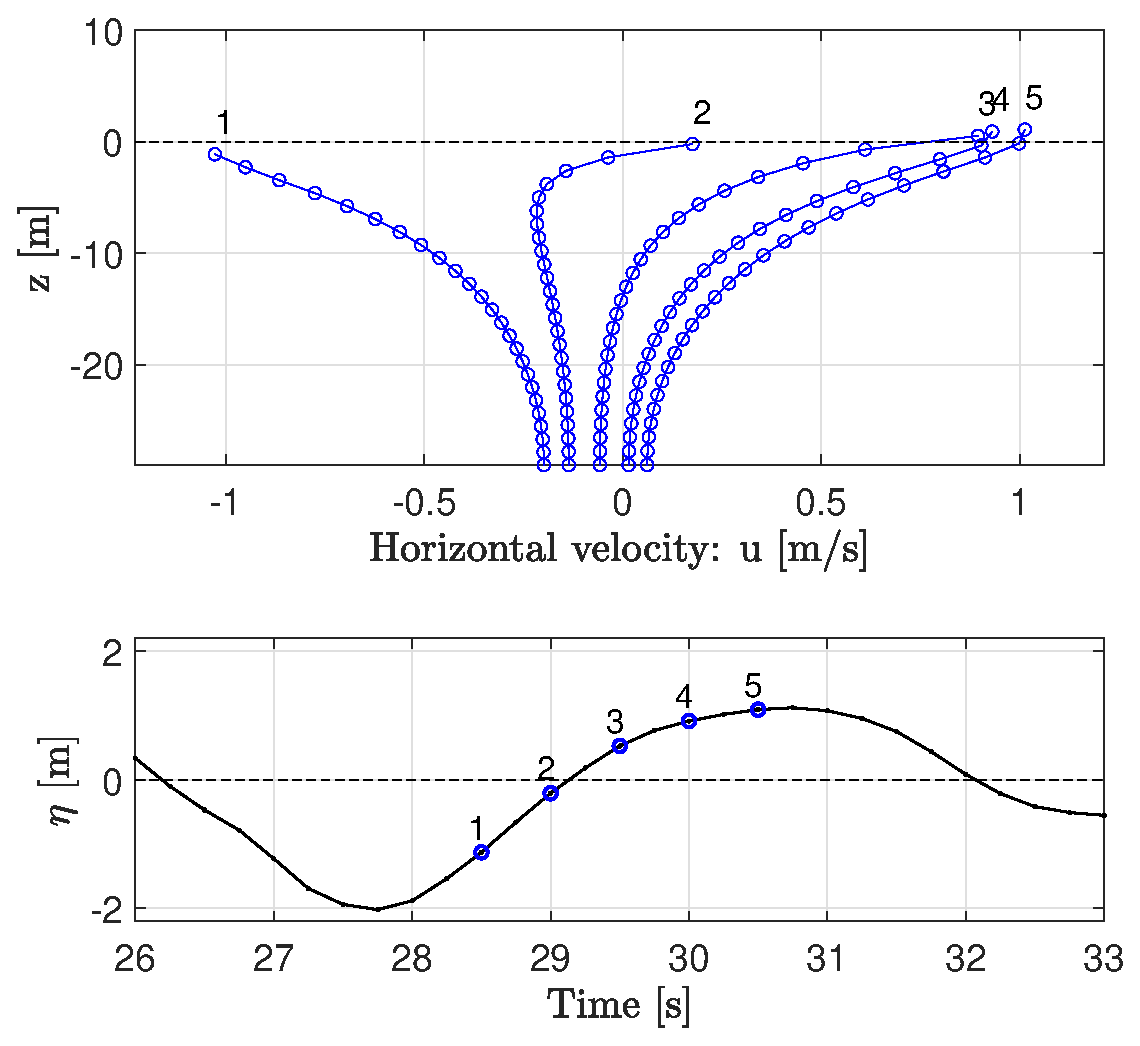
\includegraphics[width=0.7\textwidth]{Figures/Plots/etaHozvel.eps}
    \caption{Illustration of the Wheeler stretched horizontal velocity, $u$, under five different points of an arbitrary wave section from the series shown in \cref{fig:SurfaceElevation}.}
    \label{fig:etaHozvel}
\end{figure}

\paragraph{2.e)} \cref{fig:etaHozvel} presents the horizontal velocity under the wave, for five different points of an arbitrary section of the wave series (\cref{fig:SurfaceElevation}). 


\vspace{15mm}
{\let\clearpage\relax \chapter{Extension to a directional spectrum}}

\begin{figure}[htb]
\begin{subfigure}[t]{.5\textwidth}
    \centering
    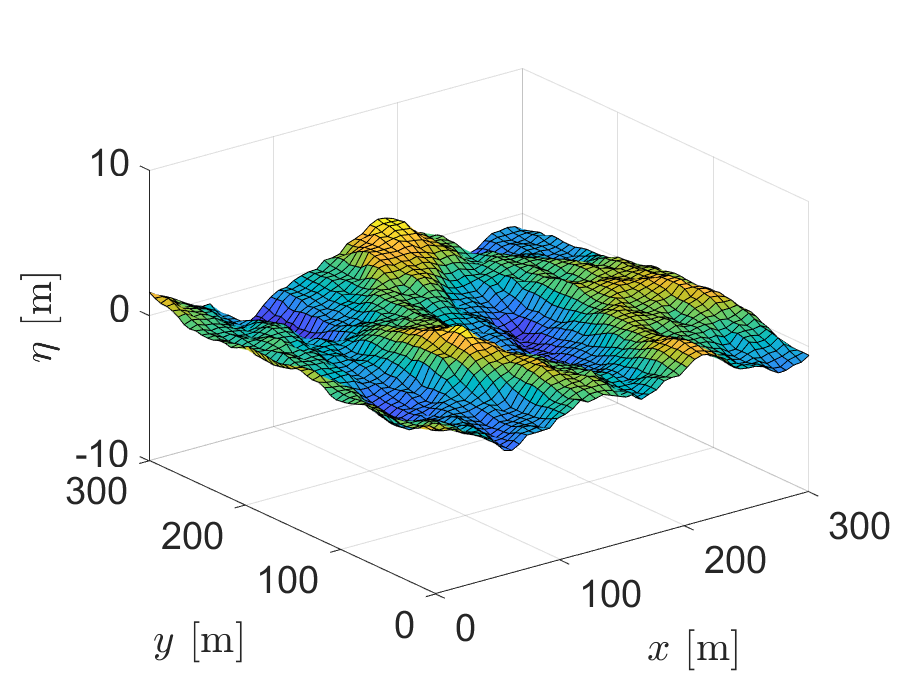
\includegraphics[width=.95\textwidth,trim=0cm 0cm 0.0cm 0cm, clip=true]{Figures/Plots/etadirns1.eps}
    \caption{No cut-off frequency $t=\SI{50}{s}$}
    \label{fig:etaIFFTdirns1}
\end{subfigure}%
\begin{subfigure}[t]{.5\textwidth}
    \centering
    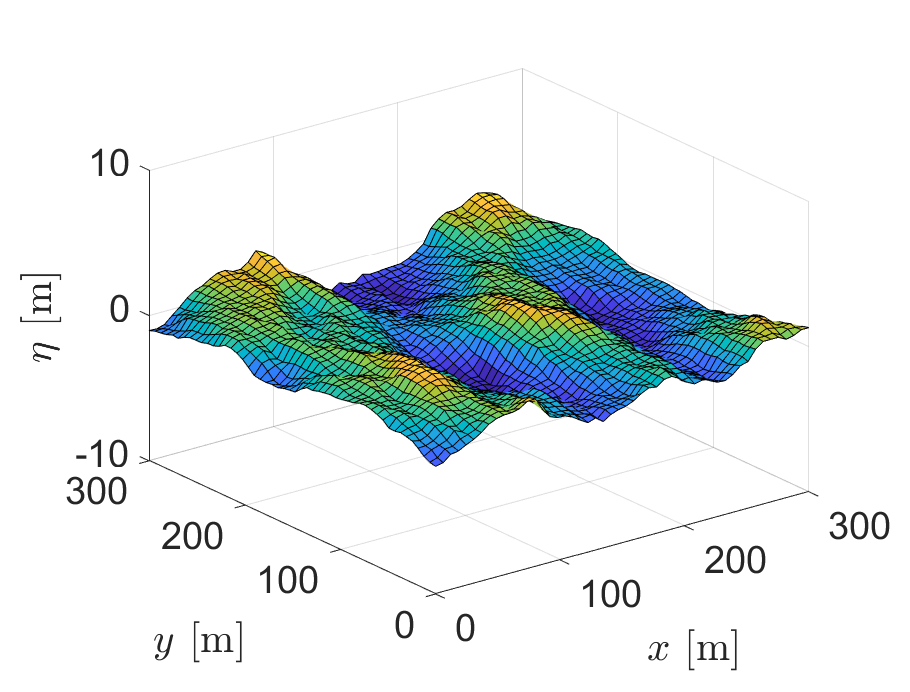
\includegraphics[width=0.95\textwidth,trim=0cm 0cm 0cm 0cm, clip=true]{Figures/Plots/etadirns2.eps}
    \caption{No cut-off frequency $t=\SI{55}{s}$}
    \label{fig:etaIFFTdirns2}
\end{subfigure}
\begin{subfigure}[t]{.5\textwidth}
    \centering
    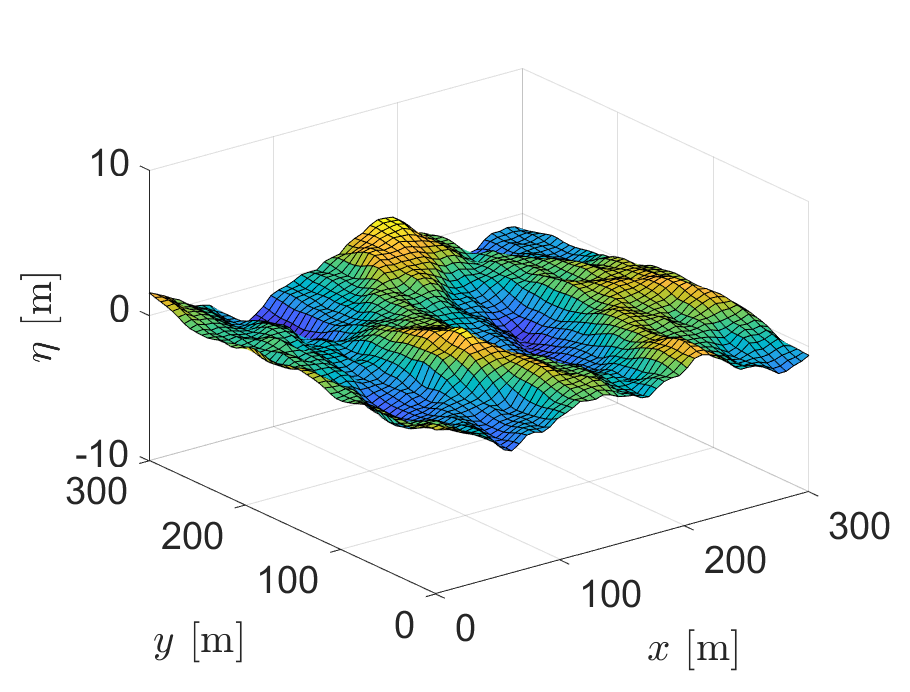
\includegraphics[width=.95\textwidth,trim=0cm 0cm 0.0cm 0cm, clip=true]{Figures/Plots/etadir1.eps}
    \caption{With cut-off frequency $t=\SI{50}{s}$}
    \label{fig:etaIFFTdir1}
\end{subfigure}%
\begin{subfigure}[t]{.5\textwidth}
    \centering
    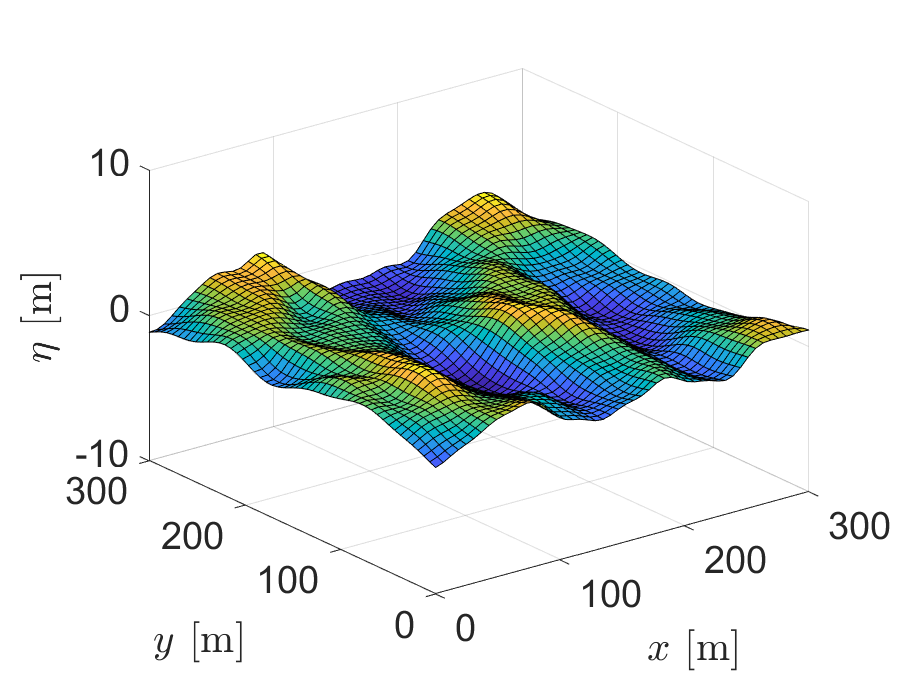
\includegraphics[width=0.95\textwidth,trim=0cm 0cm 0cm 0cm, clip=true]{Figures/Plots/etadir2.eps}
    \caption{With cut-off frequency $t=\SI{55}{s}$}
    \label{fig:etaIFFTdir2}
\end{subfigure}
\caption{Surface elevation at two times for an area of $\SI{300}{m}\times\SI{300}{m}$, with and without using a cut-off frequency of $f_{\text{cut-off}}=\SI{0.25}{Hz}$ (or period $T_{\text{cut-off}}=\SI{4}{s}$).}
\label{fig:etaIFFTdirection}
\end{figure}